% Gemini theme
% See: https://rev.cs.uchicago.edu/k4rtik/gemini-uccs
% A fork of https://github.com/anishathalye/gemini

\documentclass[final]{beamer}

% ====================
% Packages
% ====================

\usepackage[T1]{fontenc}
\usepackage{lmodern}
\usepackage[size=custom,width=120,height=72,scale=1.0]{beamerposter}
\usetheme{gemini}
% \usecolortheme{uchicago}
\usecolortheme{stanford}
\usepackage{graphicx}
\usepackage{booktabs}
\usepackage{tikz}
\usepackage{pgfplots}
\usepackage{subfig}
\usepackage{amsmath}
\usepackage{booktabs}
\usepackage{multirow}
\usepackage{float}
\pgfplotsset

% ====================
% Lengths
% ====================

% If you have N columns, choose \sepwidth and \colwidth such that
% (N+1)*\sepwidth + N*\colwidth = \paperwidth
\newlength{\sepwidth}
\newlength{\colwidth}
\setlength{\sepwidth}{0.025\paperwidth}
\setlength{\colwidth}{0.3\paperwidth}

\newcommand{\separatorcolumn}{\begin{column}{\sepwidth}\end{column}}


\title{Enhancing Game Control Through Hybrid Reinforcement Learning}


\author{Danhua Yan}

\institute[shortinst]{Department of Computer Science, Stanford University}

% ====================
% Footer (optional)
% ====================

\footercontent{
  % \href{rylanschaeffer.github.io}{rylanschaeffer.github.io} \hfill
  Stanford CS234 Default Project - Winter 2025 \hfill
  \href{mailto:dhyan@stanford.edu}{dhyan@stanford.edu}}
% (can be left out to remove footer)

% ====================
% Logo (optional)
% ====================

% use this to include logos on the left and/or right side of the header:
% \logoright{\includegraphics[height=7cm]{logos/cs-logo-maroon.png}}
% \logoleft{\includegraphics[height=7cm]{logos/cs-logo-maroon.png}}

% ====================
% Body
% ====================

\begin{document}

% This adds the Logos on the top left and top right
\addtobeamertemplate{headline}{}
{
    \begin{tikzpicture}[remember picture,overlay]
    %   \node [anchor=north west, inner sep=3cm] at ([xshift=0.0cm,yshift=1.0cm]current page.north west)
    %   {\includegraphics[height=5.0cm]{stanford_logos/Stanford-CS.png}}; % uc-logo-white.eps
      \node [anchor=north east, inner sep=3cm] at ([xshift=0.0cm,yshift=2.5cm]current page.north east)
      {
\includegraphics[height=7.0cm]{stanford_logos/Block_S_2_color.png}};
    \end{tikzpicture}
}

\begin{frame}[t]
\begin{columns}[t]
\separatorcolumn

\begin{column}{\colwidth}

  \begin{block}{Introduction}
    % what are you trying to solve? 
    % Reference current challenges and why your work is meaningful.
    \begin{itemize}
        \item \textbf{Motivation} Many environments have high-dimensional state spaces, 
        sparse rewards, and complex dynamics, making pure exploration inefficient. 
        Limited or costly exploration can prevent RL agents from learning usable policies.
        \item \textbf{Objective} This project explores hybrid RL (HRL) by combining offline 
        human demonstrations with online agent explorations to enhance game control 
        through guided exploration.
    \end{itemize}
  \end{block}

  \begin{block}{Background}
  % problem setup + notation; maybe previous work
    \begin{itemize}
      \item \textbf{Super Mario Bros.} The NES game 
      Super Mario Bros has challenges including sparse rewards, precise timing 
      for jumps, and strategy for finishing within time limits. 
      The problem is non-Markovian, requiring temporal local structure. 
      \item \textbf{Behavior Cloning (BC)} A supervised learning approach to learn 
      a policy from human demonstrated $(s,a)$ pairs.
      \item \textbf{PPO} Proximal Policy Optimization (PPO) is an RL policy 
      gradient algorithm for training intelligent agents.
      \item \textbf{Bootstrapping PPO with Guidance} PPO starts with a 
      pre-trained policy or is guided by demonstrations early in training.
    \end{itemize} 
  \end{block}
  
  \begin{block}{Methods}
  % explain your technical contributions; figures can really 
  % help understanding especially for a neural model!


  
  {\large\textcolor{cardinalred}{Data and Environment}}\noindent\vspace{-1em}
  \begin{itemize}
    \item \textbf{Human Demonstration} Script to record trajectories 
    in the same format as the RL agent, capturing controller actions 
    and game states.
    \item \textbf{Customized Environment}
    \textcolor{cardinalred}{Actions}: 3 movements.
    \textcolor{cardinalred}{Termination}: Single life and timeout terminations.
    \textcolor{cardinalred}{Rewards}: Combination of scores, time, milestones, movement to give dense rewards.
    \textcolor{cardinalred}{Sampling}: Sampled game states at 15fps to
    reduce trajectory length.
  \end{itemize}

    \begin{figure}[h]%
      \centering
      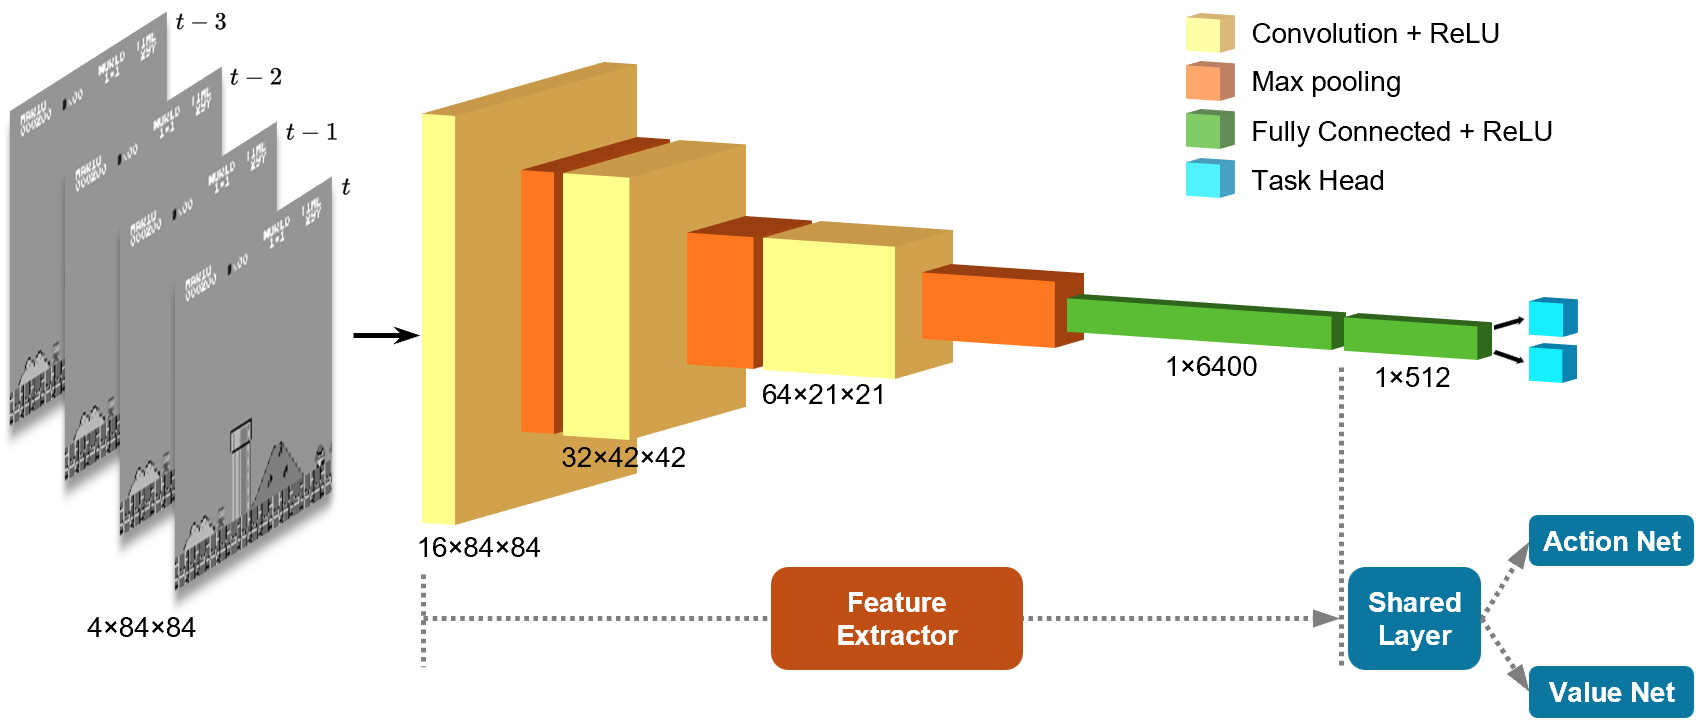
\includegraphics[width=0.8\textwidth]{pics/architecture.png}
      \caption{\textbf{PPO agent architecture for playing Super Mario Bros.}
        Four downsampled gameplay frames are stacked 
        to represent the current state $s_t$, as input to the CNN actor-critic PPO
        networks.
      }%
      \label{fig:cnn}%
  \end{figure}

  \end{block}

  % \begin{alertblock}{A highlighted block}
  % \end{alertblock}

\end{column}

\separatorcolumn

\begin{column}{\colwidth}

  % continuation of methods
  \begin{minipage}{\textwidth}
      {\large\textcolor{cardinalred}{Reinforcement Learning Models}}\noindent\vspace{-0.2em}
    
    \begin{itemize}

    \item \textbf{State Representation} Grayscale and downsampled gameplay frames. 
    State $s_t$ at time $t$ is represented by four stacked frames, 
    ${f_{t-3}, \cdots, f_t}$, preserving local temporal dynamics (see Figure. \ref{fig:cnn}).
    
    \item \textbf{Policy Network Architectures} 
    A three-layer CNN produces a 
    dense feature representation. The PPO actor-critic shares a hidden layer, 
    followed by separate action and value heads. The BC network combines the 
    feature extractor with the action head. (see Figure \ref{fig:cnn})

      \item \textbf{Baselines} Offline: BC policy on human data; 
      Online: PPO and DQN with decaying $\epsilon$-greedy.
      \item \textbf{Hybrid Reinforcement Learning (HRL)}
      \begin{itemize}
        \item \textbf{PPO Weights Pre-Training} (\texttt{HRL1}) Pre-train the policy 
        network via BC on human data, then use those weights for PPO. Evaluate different parts of the 
        actor-critic policy network transferred from BC policy (\texttt{HRL1-MLP}: action net; 
        \texttt{HRL1-FEAT}: feature extractor; \texttt{HRL1-ALL}: all weights except value head).
        \item \textbf{Assisted Explorations} (\texttt{HRL2}) Use a single human play 
        trajectory to reset PPO rollouts strategically from near the winning state back 
        to the initial state \cite{salimans2018learningmontezumasrevengesingle}. Propose 
        an exponential decay schedule where earlier states get more rollouts (\texttt{HRL2-ER}).
      \end{itemize}
    \end{itemize}
    
  \end{minipage}



  \begin{block}{Experiments}

    \begin{figure}[h]%
      \centering
      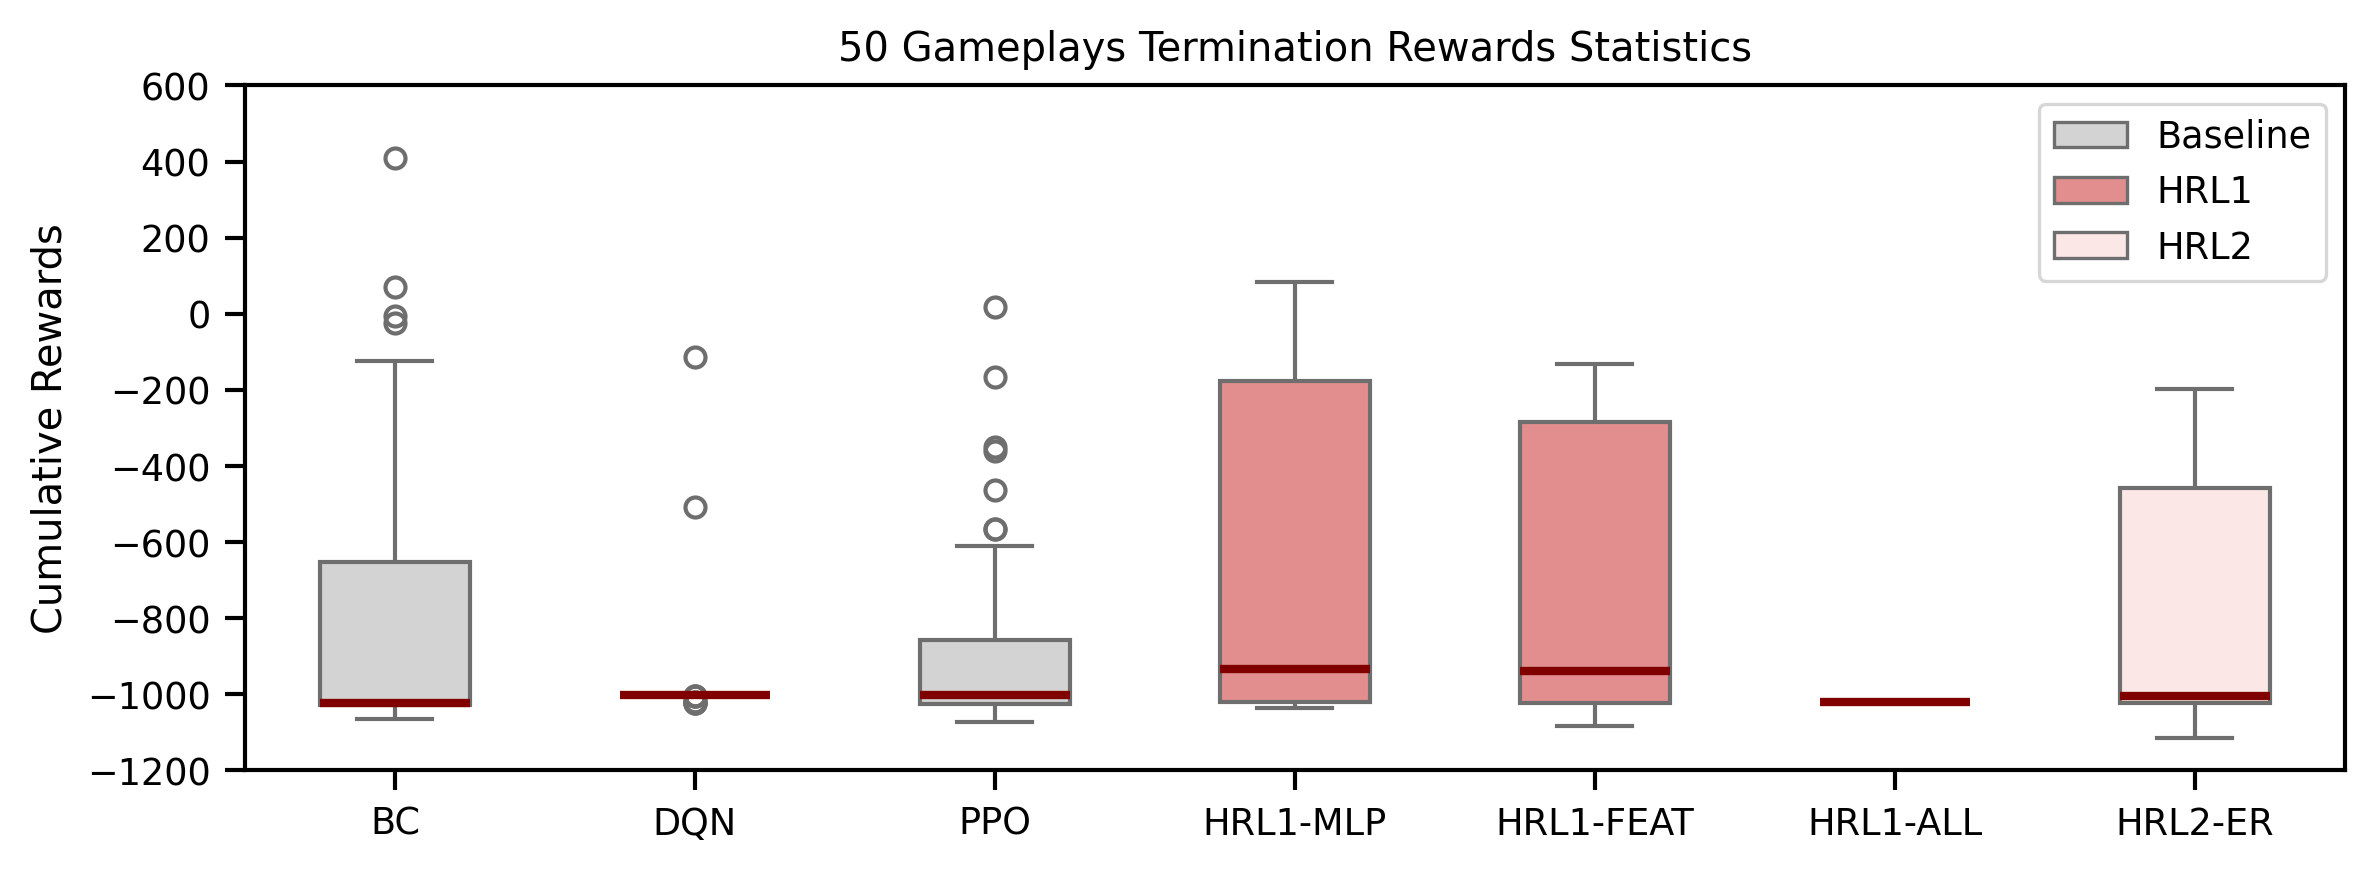
\includegraphics[width=\textwidth]{pics/cum_rewards.png}
      \caption{\textbf{Gameplay statistics of different policies.
      }}%
      \label{fig:res}%
  \end{figure}
  
  All online policies were trained for 250 rollouts to compare efficiency.
  After training, each policy was evaluated as a stochastic policy.
  We conducted 50 gameplays for each policy and compared cumulative rewards.
  
  From Figure \ref{fig:res}, we conclude: 
  \textcolor{cardinalred}{1)} Behavior cloning is a strong starting point, training faster;
  \textcolor{cardinalred}{2)} Transfer learning (\texttt{HRL1}) is effective when transferring either 
  features or actions, but not both;
  \textcolor{cardinalred}{3)} Assisted explorations (\texttt{HRL2}) offer no significant improvement 
  to the mean rewards over the PPO baseline, however higher reward distributions are observed.
    


  \end{block}

\end{column}

\separatorcolumn

\begin{column}{\colwidth}

  \begin{block}{Analysis}
    \begin{figure}[H]%
      \centering
      \subfloat[Jump over a tall pipe is the most challenging state for the level]
      {{
\includegraphics[width=0.3\textwidth]{pics/stuck pipe.png} }}%
      \hfill
      \subfloat[\texttt{HRL\_1} Policies Entropy Loss During Training]
      {{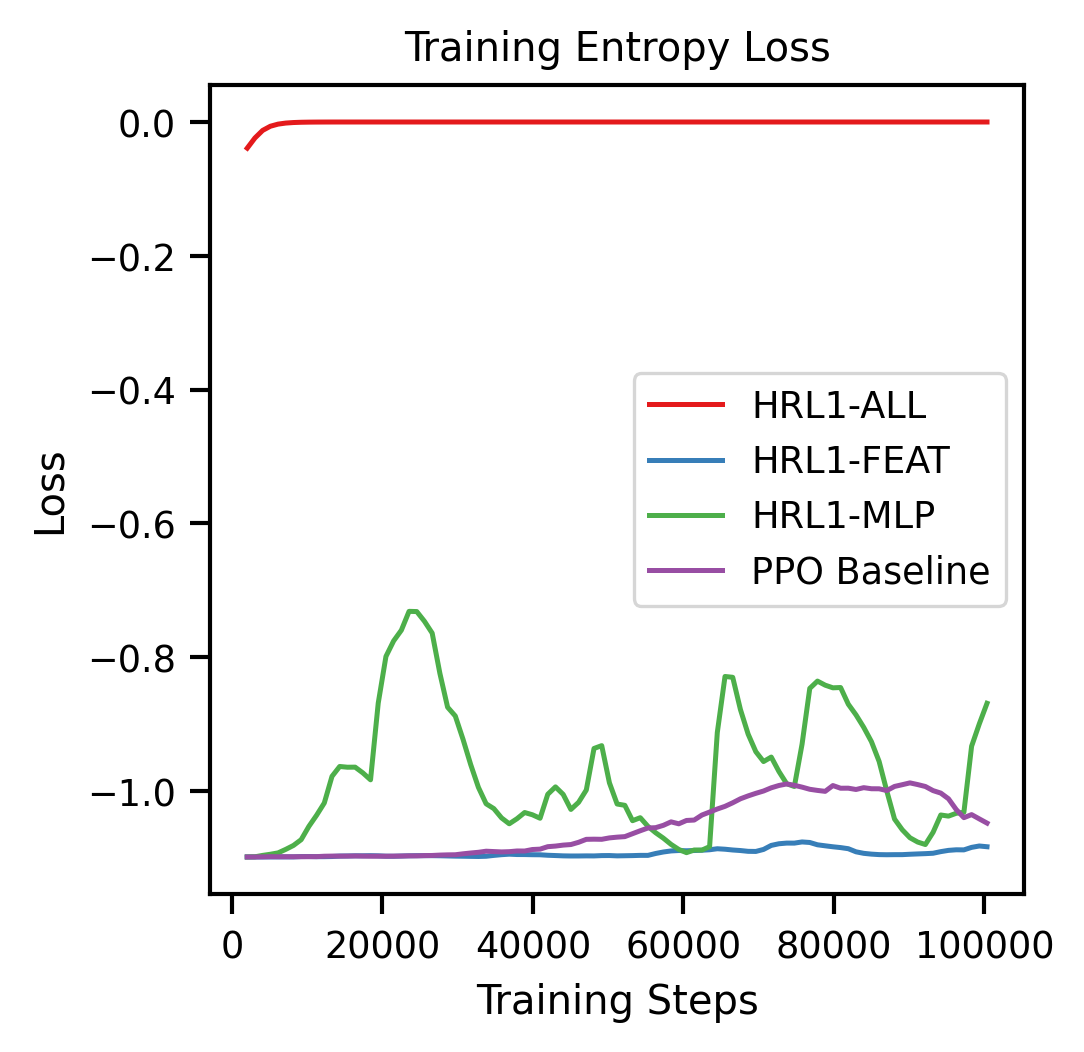
\includegraphics[width=0.3\textwidth]{pics/hrl1_ent_loss.png} }}%
      \hfill
      \subfloat[\texttt{HRL\_1} Policies Rewards During Training]
      {{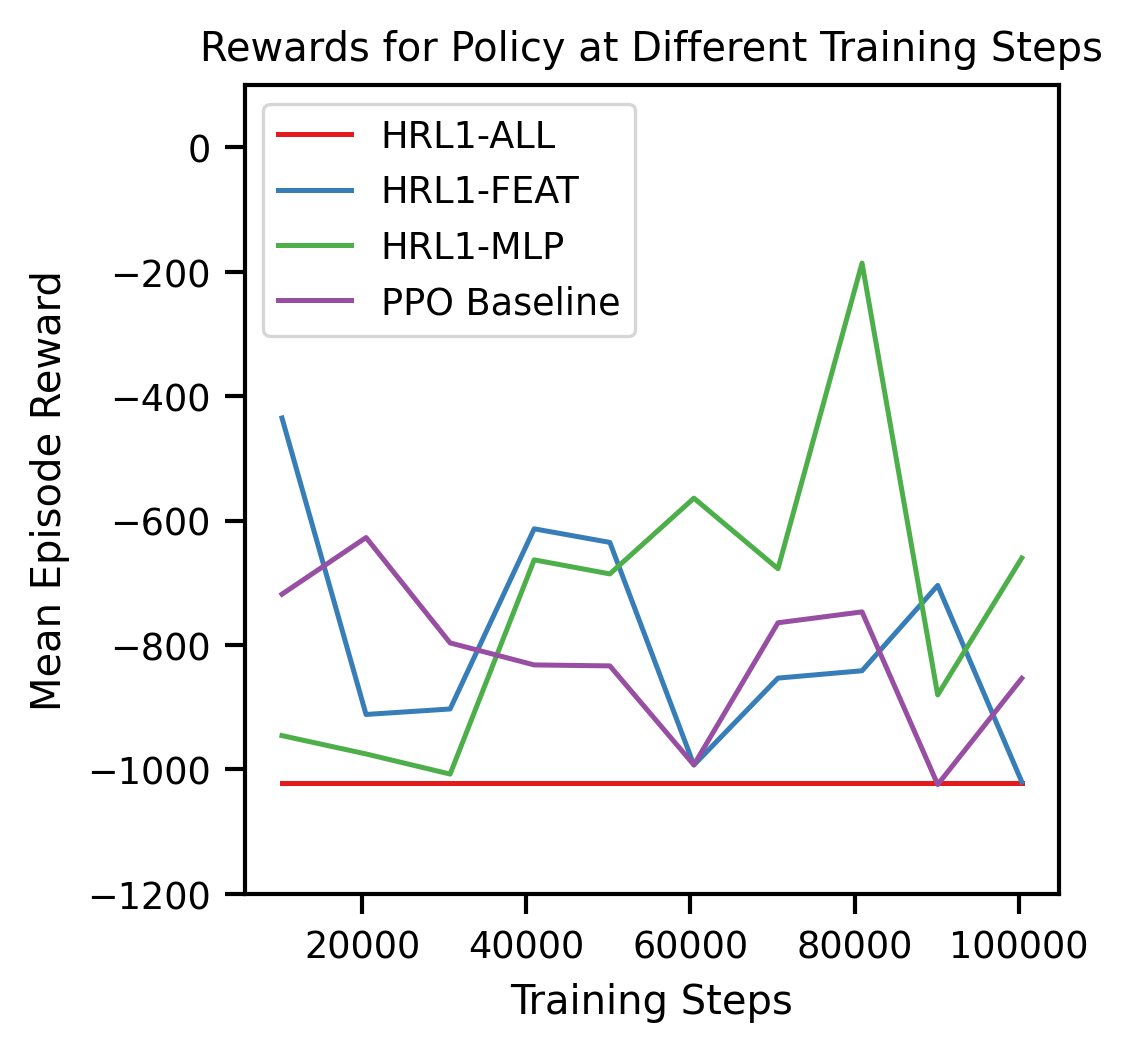
\includegraphics[width=0.3\textwidth]{pics/hrl1_eval.png} }}%
      \caption{Understanding the performance of the policies
      }%
      \label{fig:analysis}%
    \end{figure}


    All policies failed to complete the level, indicating challenges in the 
    intrinsic game mechanics and HRL algorithms.

    \begin{itemize}
      \item \textbf{Game Challenge} Level 1-1 has a tall pipe early on that 
      traps Mario. Continuous actions are required to jump over it, which 
      is difficult for the agent to learn. Temporal structure frames help, 
      but action history is also crucial. BC's randomized supervised learning 
      discards such information (see Figure \ref{fig:analysis}(a)).

      \item \textbf{PPO-Weights Pre-Training} Loading either the feature 
      extractor (\texttt{HRL1-FEAT}) or action head (\texttt{HRL1-MLP}) 
      provides a prior for state and action distributions, aiding exploration. 
      However, loading both leads (\texttt{HRL1-ALL}) to low entropy, causing PPO to stop exploring. 
      Issues with covariate shift and limited demo coverage arise, as 
      only 5 human plays with "good" states are recorded, providing little 
      information for bad states (see Figure \ref{fig:analysis}(b)(c)).

      \item \textbf{Assisted Explorations} Figure \ref{fig:res} shows that 
      assisted explorations do not improve mean rewards significantly. Mario 
      often terminates at the tall pipe (Figure \ref{fig:analysis}(a)). However, 
      once Mario passes this point, higher reward distributions are observed, 
      indicating the benefit of practicing later parts of the level without 
      rediscovering them via random exploration.
    \end{itemize}
    
  \end{block}

  \begin{block}{Conclusion}
    Behavior cloning accelerates early training, and  
    selective transfer of model components provides bootstrapping of PPO learning.  
    Future work should enhance state representations to address game challenges,
    and better demo data and algorithms are needed to mitigate covariate shift  
    and limited demo coverage.
  \end{block}

  % \begin{block}{References}
  % \noindent\rule{\textwidth}{1pt}
  \heading{Reference}
  \bibliographystyle{plain}
  \bibliography{poster}
    % \nocite{*}
    % \footnotesize{}

  % \end{block}

\end{column}

\separatorcolumn
\end{columns}
\end{frame}

\end{document}
